%!TeX root=MemoriaTFG.tex

\chapter{Contextualización}\label{contextualizacion}
% \todo{Esto es una prueba. Isaac}

Con el fin de tener una visión inicial antes de profundizar con el tema del trabajo, se explicarán brevemente los distintos conceptos que se han ido desarrollando a lo largo de la historia de la inteligencia artificial, entre ellos: definición de la inteligencia artificial, tipos de inteligencia artificial, enfoques adaptados en su desarrollo e introducción a los conceptos de las redes neuronales. ~\cite{copeland2020ai}  

\section{El mundo de la inteligencia artificial}

El concepto de \textbf{\textit{ente inteligente}} es un concepto que se lleva definiendo y redefiniendo desde hace siglos. Para los filósofos, serviría para definir la naturaleza del ser humano. Para los científicos, sería un medio por el cual se podrían llevar a cabo demostraciones lógicas impenetrables y cálculos extremadamente complejos para la resolución humana. Para los escritores, un ser fantástico y poderoso capaz de realizar cosas inimaginables, a menudo despertando el miedo en los lectores. \\

Sin embargo, en su esencia, es una \textit{expansión de las capacidades humanas}, una mejora, un mecanismo de resolución de tareas y problemas que facilitaría la vida en todos sus aspectos.~\cite{buchanan2005very}

\subsection{¿Qué es la inteligencia artificial?}

La inteligencia artificial se define como la \textbf{capacidad de una máquina de simular el comportamiento y el razonamiento humano}, de tal manera que frente a cualquier situación razone y/o actúe de la misma manera que una persona haría. \\

La inteligencia humana está compuesta de tres tipos de ingeligencia distintas, algo de lo que Santiago Sánchez-Migallón, profesor de filosofía y colaborador en Xataka, explicaba en un interesante repaso de $"$\textit{qué hace al ser humano inteligente}$"$: \cite{pastor2008inteligencia}

\begin{enumerate}
    \item \textbf{Inteligencia componencial}, nuestra capacidad de análisis: dirección consciente de nuestros procesos mentales para analizar y evaluar ideas, resolver problemas y tomar decisiones.
    \item \textbf{Inteligencia experiencial}, nuestra creatividad: capacidad de afrontar tareas novedosas, formular nuevas ideas y combinar experiencias.
    \item \textbf{Inteligencia práctica o contextual}, capacidad de adaptación al medio: adaptación, selección o modificación del ambiente individual. Realmente, esta es la inteligencia más importante (si bien depende de las otras dos), ya que tu éxito o fracaso  dependerá de ella. 
\end{enumerate}


Para que una máquina sea inteligente, esta debe: 

\begin{enumerate}
    \item Tener la habilidad de \textbf{\textit{razonar}}. El razonamiento puede ser \textbf{inductivo} o \textbf{deductivo}:
        \begin{enumerate}
            \item En el razonamiento deductivo la veracidad de las premisas \textit{garantiza} la veracidad de la conclusión
            \item En el razonamiento inductivo las premisas verdaderas \textit{apoyan} la veracidad de la conclusión pero sin asegurarla
        \end{enumerate}
    \item Poder \textbf{\textit{analizar}} el entorno, \textbf{\textit{entender las percepciones}} recibidas y, a partir de éstas, \textbf{\textit{determinar cómo debe actuar o comportarse a continuación}}
    \item \textbf{\textit{Aprender de experiencias}} anteriores, de tal manera que tenga memoria de todas las interacciones que ha llevado a cabo 
    \item A partir de la experiencia, ser capaz de \textbf{\textit{generalizar conceptos}}; es decir, ser capaz de realizar conexiones de causa y consecuencia, reglas internas que expliquen el por qué de las percepciones que recibe y ser capaz de reconocer las percepciones que son iguales
\end{enumerate}

\subsection{Tipos de inteligencia artificial}

Según Stuart Russell y Peter Norvig, autores del aclamado libro \textit{Inteligencia Artificial: Un enfoque moderno}, hay 4 tipos distintos de inteligencia artificial:
\begin{enumerate}
    \item Sistemas que \textbf{\textit{piensan} como humanos} - estos sistemas tratan de reproducir el pensamiento humano. A esta categoría pertenecen las redes neuronales artificiales. Entre las actividades que se pueden llevar a cabo con estos sistemas son la toma de decisiones, la resolución de problemas y el aprendizaje.
    \item Sistemas que \textbf{\textit{actúan} como humanos} - estos sistemas tratan de imitar el comportamiento humano. Un ejemplo de sistemas de este tipo es la robótica.
    \item Sistemas que \textbf{\textit{piensan} racionalmente} - estos sistemas tratan de imitar o emular el pensamiento lógico racional del ser humano. Un ejemplo de estos sistemas son los sistemas expertos (como MYCIN).
    \item Sistemas que \textbf{\textit{actúan} racionalmente} - tratan de emular de forma racional el comportamiento humano. A esta última categoría pertenecen los agentes inteligentes, y es el tipo de inteligencia artificial que se ha estado desarrollando para el TFG.
\end{enumerate}

\subsection{Enfoques de la inteligencia artificial}

Existen dos tipos de enfoques que se siguen cuando se desea implementar un sistema inteligente:
\begin{enumerate}
    \item Simbólico, o \textit{\textbf{descendente}}: se quiere replicar la inteligencia mediante premisas definidas. Según la hipótesis formulada por Newell y Simon (\textit{physical symbol system hypothesis}) \cite{nilsson2007physical}, \textit{$"$el procesamiento de estructuras de símbolos es suficiente, teóricamente, para producir inteligencia artificial en un ordenador digital y que, además, la inteligencia humana es el resultado del mismo tipo de manipulación simbólica.$"$}
    \item Conexionista, o \textit{\textbf{ascendente}}: se pretende emular las capacidades y el comportamiento del cerebro humano mediante procesos que emergen de redes formadas por unidades sencillas interconectadas (como las neuronas). Las redes neuronales artificiales han sido creadas para que repliquen las conexiones del cerebro humano, de ahí el término \textit{conexionista}. En la siguiente sección se explicará más detenidamente este enfoque. 
\end{enumerate}

El enfoque descendente ofrece buenos resultados en ámbitos poco complejos pero suelen estancarse cuando se les presenta situaciones reales; esto se debe a que es imposible recoger todas las combinaciones de las percepciones y sus correspondientes respuestas. \\

Por otro lado, el enfoque ascendente tiene problemas en replicar el sistema nervioso de incluso seres vivos simples. El cerebro es y continuará siendo una incógnita hasta que se consiga replicar artificialmente y, de esta manera, estudiar todos los procesos que se llevan a cabo al realizar acciones como pensar, recordar, aprender, etc. 

\section{Conexionismo}

El conexionismo, o la \textit{computación neuronal}, se ha desarrollado como un intento de entender cómo funciona el cerebro humano a nivel neuronal y, más concretamente, cómo las personas \textit{aprenden} y son capaces de \textit{recordar}. \\

En 1943, el neurólogo Warren McCulloch y el matemático Walter Pitts publicaron un trabajo sobre las redes neuronales en el cual se exponía que una neurona del cerebro \textbf{es como un procesor digital}, y que el cúmulo de éstas componen \textbf{una máquina computacional}; al fin y al cabo, el cerebro es un sistema que \textit{calcula} acciones que el humano debe tomar. As McCulloch put it subsequently, “What we thought we were doing (and I think we succeeded fairly well) was treating the brain as a Turing machine.”

\subsection{Creación de una red neuronal}

La primera red neuronal fue creada años después, en 1954 (Belmont Farley y Wesley Clark). Contaba con un \textbf{total de 128 neuronas y era capaz de reconocer patrones sencillos}. Además, se descubrió que aunque se eliminen menos del 10\% del total de neuronas de la red entrenada, su eficacia y rendimiento no se verían afectados; este hecho recuerda a cómo el cerebro puede sufir daños leves tras sufrir una operación, un accidente o una enfermedad y mantener sus capacidades. \\

\begin{figure*}[h]
    \centering
    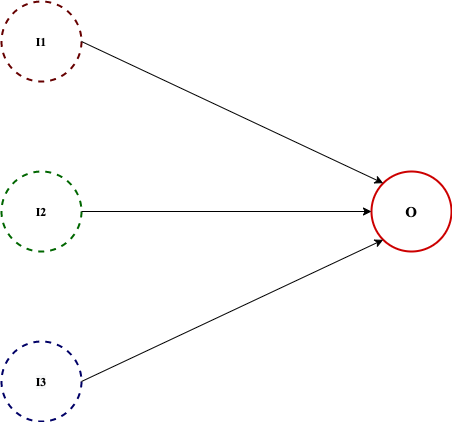
\includegraphics[scale=0.35]{cap2_contextualizacion/images/red_neuronal.png}
    \caption{Red neuronal simple}
    \label{fig:red_neuronal_simple}
\end{figure*}

En la figura \ref{fig:red_neuronal_simple} se muestra una simple red neuronal que consta de 4 neuronas - las neuronas \textbf{\textit{I1}}, \textbf{\textit{I2}} e \textbf{\textit{I3}} corresponden a las neuronas de entrada (\textit{input}) y todas se conectan a la neurona \textbf{\textit{O}}, la neurona de salida (\textit{output}). \\

El funcionamiento de una red neuronal es sencillo - la información se va transfiriendo por las neuronas por medio de \textit{estímulos} que van activando o desactivando las neuronas que componen la red. Para que una neurona \textbf{se active} (también se hace el símil de que la neurona se \textit{dispara}), debe recibir unos estímulos de las neuronas a las que ya están conectadas. La neurona por su lado interpreta este estímulo y, a su vez:

\begin{enumerate}
    \item Se activa (1) y estimula a las siguientes neuronas a las que está conectada
    \item Permanece desactivada (0) y se acaba la interacción 
\end{enumerate}

Un estímulo de una neurona se calcula \textbf{teniendo en cuenta todas las neuronas} activas que están conectadas a la neurona de salida (es decir, la que se desea activar a continuación). Cada conexión entre las neuronas de entrada y salida tiene un peso $\omega$, y la suma ponderada de los pesos es el estímulo total. Para que una neurona se active este estímulo debe ser mayor o igual al umbral de activación $\theta$ de la neurona. \\

Para poder poner un ejemplo se considerará que:

\begin{enumerate}
    \item La neurona O tendrá un umbral de activación de \textbf{4}
    \item La conexión entre la neurona \textit{I1} y la \textit{O} tiene un peso de \textbf{1}
    \item El peso entre la \textit{I2} y \textit{O} es \textbf{2.75}
    \item El peso entre \textit{I3} y \textit{O} es \textbf{0.25}
\end{enumerate} 

En la figura [\ref{fig:red_neuronal_activacion}] se plantean 2 casos distintos: 

\begin{enumerate}
    \item Las neuronas \textit{I1} e \textit{I2} están activas pero la \textit{I3} está inactiva. La suma ponderada de los pesos está por debajo del umbral de activación de la neurona \textit{O}, por lo que no se activará. [\ref{fig:red_neuronal_inactiva}]
    \item Todas las neuronas están activas y la suma ponderada de los pesos es igual al umbral de activación de \textit{O}, por lo que ésta se activará. [\ref{fig:red_neuronal_activa}]
\end{enumerate}

\begin{figure}[h]
    \centering
    \begin{subfigure}{.45\textwidth}
        \centering
        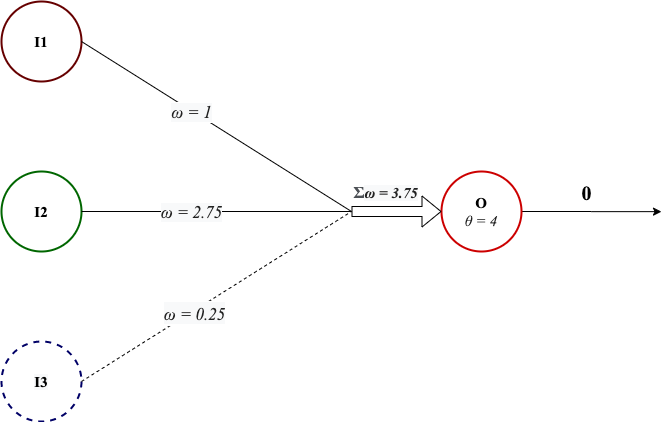
\includegraphics[scale=0.22]{cap2_contextualizacion/images/red_neuronal_inactive.png}
        \caption{I3 inactivo, suma ponderada por debajo del umbral de activación de O}
        \label{fig:red_neuronal_inactiva}
    \end{subfigure}      
    \begin{subfigure}{.45\textwidth}
        \centering
        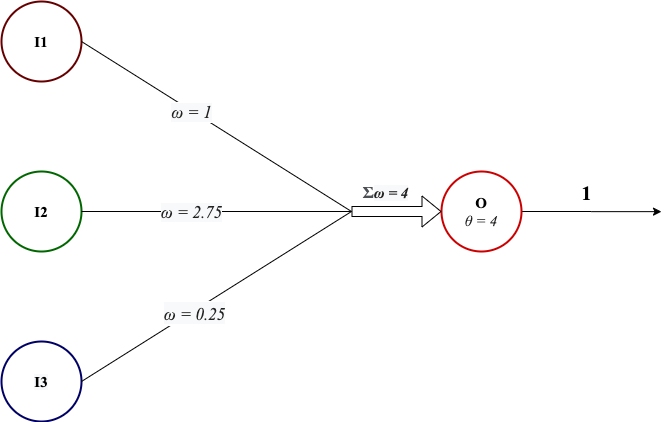
\includegraphics[scale=0.22]{cap2_contextualizacion/images/red_neuronal_active.png}
        \caption{I1, I2, I3 activas, suma ponderada igual al umbral de activación de O}
        \label{fig:red_neuronal_activa}
    \end{subfigure}
    \caption{Activación de la neurona O según las neuronas activas de entrada}
    \label{fig:red_neuronal_activacion}
\end{figure}

\subsection{Entreno de una red neuronal}

Las redes neuronales son ampliamente usadas en las tareas de predicción y de clasificación. Sin embargo, como paso previo a estas tareas es necesario \textit{\textbf{entrenar}} la red. El proceso de entreno sirve para que la red \textit{adquiera experiencia} con los datos, de modo que será capaz de reconocer, clasificar y/o predecir el resultado adecuado con cada dato que se le presenta. \\

En el entreno es necesario disponer de un \textit{conjunto de datos de entrenamiento}. Este \textit{dataset} estará compuesto por distintas muestras - parejas de datos de entrada y de salida con las que la red aprenderá cuáles son las interpretaciones correctas. \\

En cuanto al proceso, el entreno consiste en los siguientes pasos: 
\begin{enumerate}
    \item El agente externo presenta un ejemplo de patrón a la red y observa el comportamiento de \textit{O}
    \item El agente ajusta los pesos de las conexiones en función de estas dos normas:
        \begin{enumerate}
        \item Si el resultado es 0 pero se deseaba una salida de 1, se \textbf{incrementa} el peso de todas las conexiones de las neuronas \textit{activas} que conducen a O (y así se incrementa las probabilidades de que O se active cuando se presenten las mismas condiciones)
        \item Si el resultado es 1 pero se deseaba una salida de 0, se \textbf{decrementa} el peso de todas las conexiones de las neuronas \textit{activas} que conducen a O (y así se incrementa las probabilidades de que O se active cuando se presenten las mismas condiciones)
    \end{enumerate}
\end{enumerate}

Este proceso se realiza varias iteraciones, en cada iteración aplicando este proceso de dos paso a cada muestra del \textit{dataset}. De esta manera se obtiene un \textit{patrón de pesos} de conexiones que permite que la red responda con la salida correcta para todos los ejemplos ofrecidos. \\

\section{Machine Learning. El aprendizaje en inteligencia artificial}


\textbf{\textit{Machine Learning}} o \textit{Aprendizaje automático} hace referencia a la capacidad de una máquina, software u aplicación de aprender mediante la aplicación de algoritmos específicos a cierta entrada de datos de su sistema de manera independiente. \cite{apd2019ml}

\subsubsection{¿Qué es Machine Learning?}
El \textbf{Aprendizaje Automático} consiste en una disciplina de las ciencias informáticas, relacionada con el desarrollo de la Inteligencia Artificial, y que sirve, como ya se ha dicho, para crear sistemas que pueden aprender por sí solos. \\

Es una tecnología que permite hacer automáticas una serie de operaciones con el fin de reducir la necesidad de que intervengan los seres humanos. Como estas acciones se realizan de manera autónoma por el sistema, se dice que el aprendizaje es \textit{automático}.\\

El aprendizaje es la capacidad del sistema para identificar una gran serie de patrones complejos determinados por una extensa cantidad de parámetros. Para que aprenda, el algoritmo interno del sistema se modifica con la constante entrada de datos en la interfaz, y puede, de ese modo, predecir escenarios futuros o tomar acciones de manera automática según ciertas condiciones.

\subsubsection{¿Cómo funciona el Machine Learning?}
En los inicios de la informática el único modo de conseguir que un sistema hiciera algo era escribiendo un algoritmo que definiera el contexto y detalles de cada acción, por lo que el proceo estaba completamente supervisado y controlado por un ser humano. \\

En cambio, los algoritmos que se usan en el desarrollo del \textit{Machine Learning} realizan buena parte de estas acciones por su cuenta. Obtienen sus propios cálculos según los datos que se recopilan en el sistema, y cuantos más datos obtienen, mejores y más precisas serán las acciones resultantes. \\

El éxito de un buen sistema de aprendizaje automático se encuentra en la construcción y adaptación de los árboles de decisiones en base a los datos previamente conocidos por el sistema. Sin embargo, también influye la \textbf{aplicación de fórmulas heurísticas} en los nodos que forman el árbol mediante las que elabora un sistema de inferencias. \\

El sistema de Machine Learning \textbf{necesita contar con un volumen de datos de relevancia para poder suministrar respuestas realmente válidas}. Es decir, cuantos más datos tiene para entrenar y con los que aprender, mejores predicciones, clasificaciones, análisis, etc. será capaz de realizar. Al igual que en la estadística clásica, cuantos más muestras se tenga de la población más se podrá generalizar y crear un sistema que sea capaz de reconocer el mayor número de casos posibles. 

\subsection{Tipos de aprendizaje}

Un sistema de aprendizaje automático utiliza sus experiencias y las evidencias de su entorno como datos para identificar y analizar por sí mismo patrones, comportamientos, relaciones del entorno, etc. De esta manera, adquiere una capacidad de elaborar predicciones de escenarios o iniciar operaciones que son la solución para una tarea específica. \\

A partir de un gran número de ejemplos de un mismo escenario \textbf{se puede elaborar un modelo que deduzca y generalice el comportamiento observado}. \textbf{Una vez construido el modelo se podrán realizar predicciones para casos totalmente nuevos}. \\

En la sección anterior se ha explicado brevemente cómo se prepara y entrena una red que sigue un \textit{aprendizaje supervisado}. El entreno al fin y al cabo es la forma que tiene la red de \textbf{aprender}, de convertirse en \textit{inteligente}. El aprendizaje en inteligencia artificial es uno de los pilares más importantes, y existen tres categorías distintas: el \textbf{aprendizaje supervisado}, el \textbf{aprendizaje no supervisado}, y el \textbf{aprendizaje por refuerzo}. En la figura \ref{fig:ml_tipos_aprendizaje} se muestran todas las aplicaciones de cada uno de los aprendizajes. 
 
\begin{figure*}[h]
    \centering
    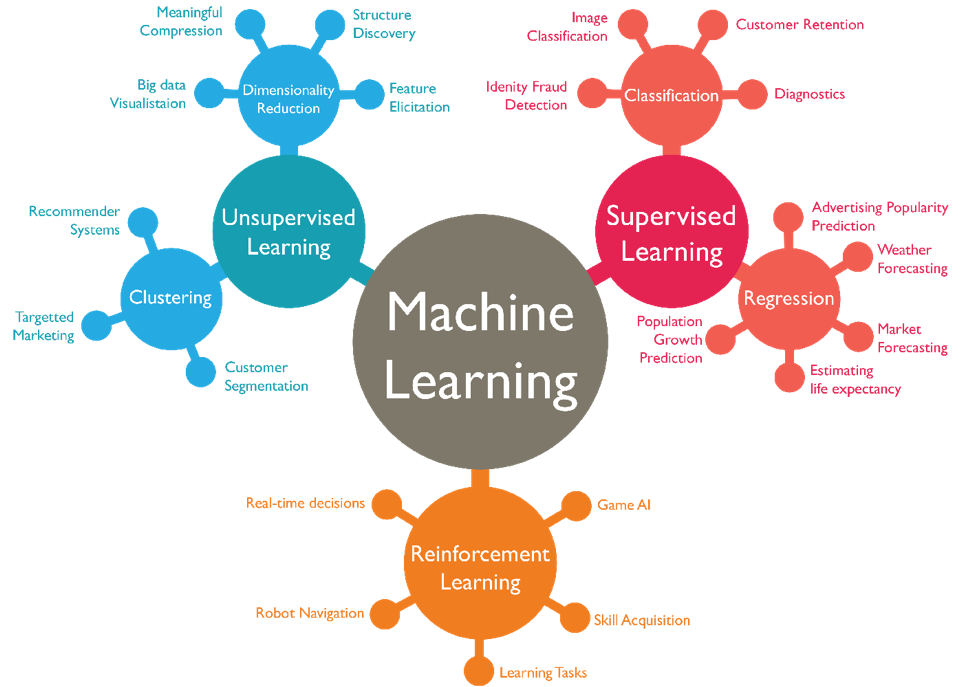
\includegraphics[scale=0.5]{cap2_contextualizacion/images/ml_learning.png}
    \caption{Tipos de aprendizaje en Machine Learning \cite{chugh2008mltypes}}
    \label{fig:ml_tipos_aprendizaje}
\end{figure*}


\subsubsection{Aprendizaje supervisado}

El \textit{aprendizaje supervisado} se basa en la existencia de \textbf{\textit{muestras etiquetadas}} con las que el modelo \textbf{aprende a identificar} los distintos ejemplos que se los proporciona \textbf{por sus etiquetas}: aprende a \textit{clasificarlos}. Para hacer un símil con la naturaleza humana, es como estar enseñándole un objeto a un niño  y diciéndole qué es para que lo pueda reconocer en un futuro. \\

Una vez que se le ha proporcionado la suficiente cantidad de dichos datos, podrán introducirse nuevos datos sin necesidad de etiquetas, en base a patrones distintos que ha venido registrando durante el entrenamiento. Este sistema se conoce como \textbf{\textit{clasificación}}. \\

Otro método de desarrollo del Aprendizaje Automático consiste en predecir un valor continuo, utilizando parámetros distintos que, combinados en la introducción de nuevos datos, permite predecir un resultado determinado. Este método se conoce como \textbf{\textit{regresión}}. \\

Lo que distingue al Aprendizaje Supervisado es que se utilizan distintos ejemplos a partir de los que generalizar para nuevos casos. \\

\subsubsection{Aprendizaje no supervisado}

En cambio, en el \textit{aprendizaje no supervisado} se entrena con datos sin etiquetas - el modelo analiza los datos y se crea él sus propias etiquetas, sus propios grupos, según distintos estrategias de análisis (por distancia, generalmente). \\

Estos sistemas tienen como finalidad la comprensión y abstracción de patrones de información de manera directa, concepto que se conoce como \textbf{\textit{clustering}}.

Este tipo de aprendizaje es más complejo que el anterior, pero es capaz de encontrar relaciones y patrones en los datos que los humanos no serían capaces de reconocer. \\

Un ejemplo de aplicación de este aprendizaje es la clasificación de los compradores en base a sus intereses y a su historial de compras. Este análisis podría mostrar una relación entre la información demográfica de una persona y sus tendencias de compras. \\

\begin{figure*}[h]
    \centering
    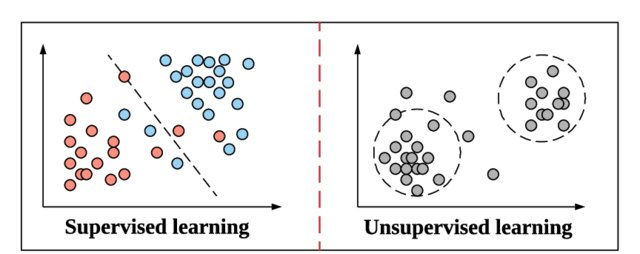
\includegraphics[scale=1]{cap2_contextualizacion/images/diff_sup_unsu.jpg}
    \caption{Aprendizaje supervisado vs. no supervisado}
    \label{fig:diff_sup_unsu}
\end{figure*}

\subsubsection{Aprendizaje por refuerzo}

En la técnica de \textit{aprendizaje por refuerzo} el aprendizaje se realiza por medio de la \textbf{\textbf{prueba y error}}, por lo que los sistemas aprenden completamente a partir de la experiencia - sin intervenciones humanas ni datos con etiquetas. Mediante el uso de funciones de premio que optimizan su comportamiento, el sistema se consigue ser \textbf{\textit{totalmente autónomo}}. \\

A modo de resumen, en la figura \ref{fig:ml_ceralytics} se puede observar un ejemplo de cómo sería entrenar un robot:

\begin{itemize}
    \item En el aprendizaje supervisado se le dice al robot que el objeto es un cubo y éste lo memoriza.
    \item En el aprendizaje no supervisado al robot se le dan dos tipos de piezas y los divide en grupos según su forma.
    \item En el aprendizaje por refuerzo el robot no tiene ninguna información externa pero mediante las percepciones (las formas del hueco y de la figura) y las interacciones (intentar introducir la figura en ambos huecos y ver si entra o no) con su entorno llegará, con el tiempo, a reconocer en qué hueco debe ir la pieza.
\end{itemize}
\begin{figure*}[h]
    \centering
    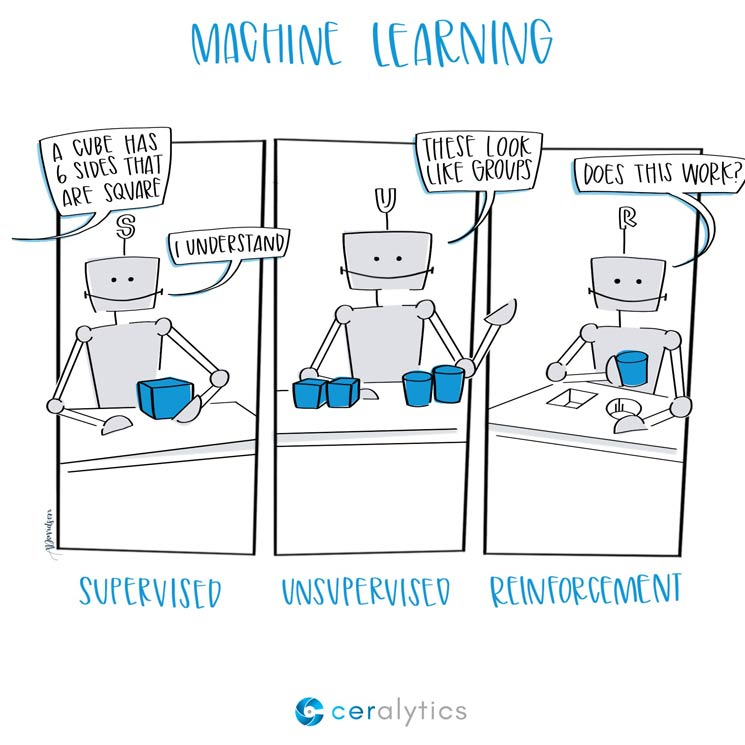
\includegraphics[width=0.45\textwidth]{cap2_contextualizacion/images/machine-learning_ceralytics.jpg}
    \caption{Cómo se diferencian los distintos tipos de aprendizaje en Machine Learning \cite{ceralyticsMLtypes}}
    \label{fig:ml_ceralytics}
\end{figure*}
\subsection{Reinforcement Learning}

El trabajo realizado se basa en el tercer tipo de aprendizaje: \textbf{el aprendizaje por refuerzo}. En este tipo de aprendizaje, la información con la que se entrena al modelo se adquiere mediante las distintas interacciones que el sistema tiene con el entorno del problema dado. \\

Las interacciones vienen definidas, de tal manera que se conoce para cada una de ellas qué efecto tendrá en el entorno, pero no está definido su significado. La manera de discriminar y de enseñarle al sistema que se ha realizado la interacción adecuada para alcanzar su objetivo se hace mediante refuerzos, o como también se les conoce, las \textbf{recompensas}. 